% Figure after Kjell Magne Fauske
% http://www.texample.net/tikz/examples/neural-network/
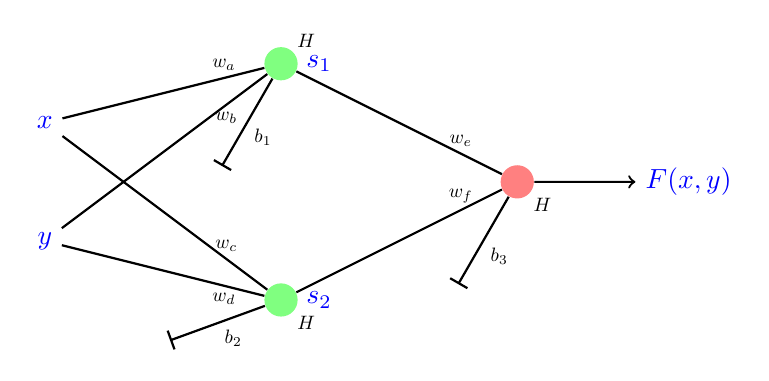
\begin{tikzpicture}[scale=1.5]
   \def\layersep{2cm}
    \tikzstyle{every pin edge}=[thick]
    \tikzstyle{neuron}=[circle,fill=black!25,minimum size=12pt,inner sep=0pt]
    \tikzstyle{entree}=[];
    \tikzstyle{input neuron}=[neuron, fill=green!50];
    \tikzstyle{output neuron}=[neuron, fill=red!50];
    \tikzstyle{hidden neuron}=[neuron, fill=blue!50];
    \tikzstyle{annot} = [text width=4em, text centered]

% Entree
\node[entree,blue] (E-1) at (-\layersep,-1) {$x$};
\node[entree,blue] (E-2) at (-\layersep,-2) {$y$};

% Premiere couche
\node[input neuron] (I-1) at (0,-0.5) {};
\node[input neuron] (I-2) at (0,-2.5) {};

\node[above right=0.8ex,scale=0.7] at (I-1) {$H$};
\node[below right=0.8ex,scale=0.7] at (I-2) {$H$};

\node[right=1.3ex,blue] at (I-1) {$s_1$};
\node[right=1.3ex,blue] at (I-2) {$s_2$};

%Seconde couche et sortie
\node[output neuron] (O) at (\layersep,-1.5 cm) {};
\node[below right=0.8ex,scale=0.7] at (O) {$H$};

% Arrete et poids
 \path[thick] (E-1) edge node[pos=0.8,above,scale=0.7]{$w_a$} (I-1) ;
 \path[thick] (E-2) edge node[pos=0.8,below,scale=0.7]{$w_b$} (I-1);
 \draw[-|,thick] (I-1) to node[midway,below right,scale=0.7]{$b_1$} ++ (-120:1);

 \path[thick] (E-1) edge node[pos=0.8,above,scale=0.7]{$w_c$} (I-2);
 \path[thick] (E-2) edge node[pos=0.8,below,scale=0.7]{$w_d$} (I-2);
 \draw[-|,thick] (I-2) to node[midway,below right,scale=0.7]{$b_2$} ++ (-160:1);

 \path[thick] (I-1) edge node[pos=0.8,above,scale=0.7]{$w_e$} (O);
 \path[thick] (I-2) edge node[pos=0.8,above,scale=0.7]{$w_f$}(O);
 \draw[-|,thick] (O) to node[midway,below right,scale=0.7]{$b_3$} ++ (-120:1) ;

% Sortie
 \draw[->,thick] (O)-- ++(1,0) node[right,blue]{$F(x,y)$};

\end{tikzpicture}  